% LaTeX code for including figures in the paper

% Figure for Section 4 (Isomorphisms Between the Three Approaches)
\begin{figure}[htbp]
  \centering
  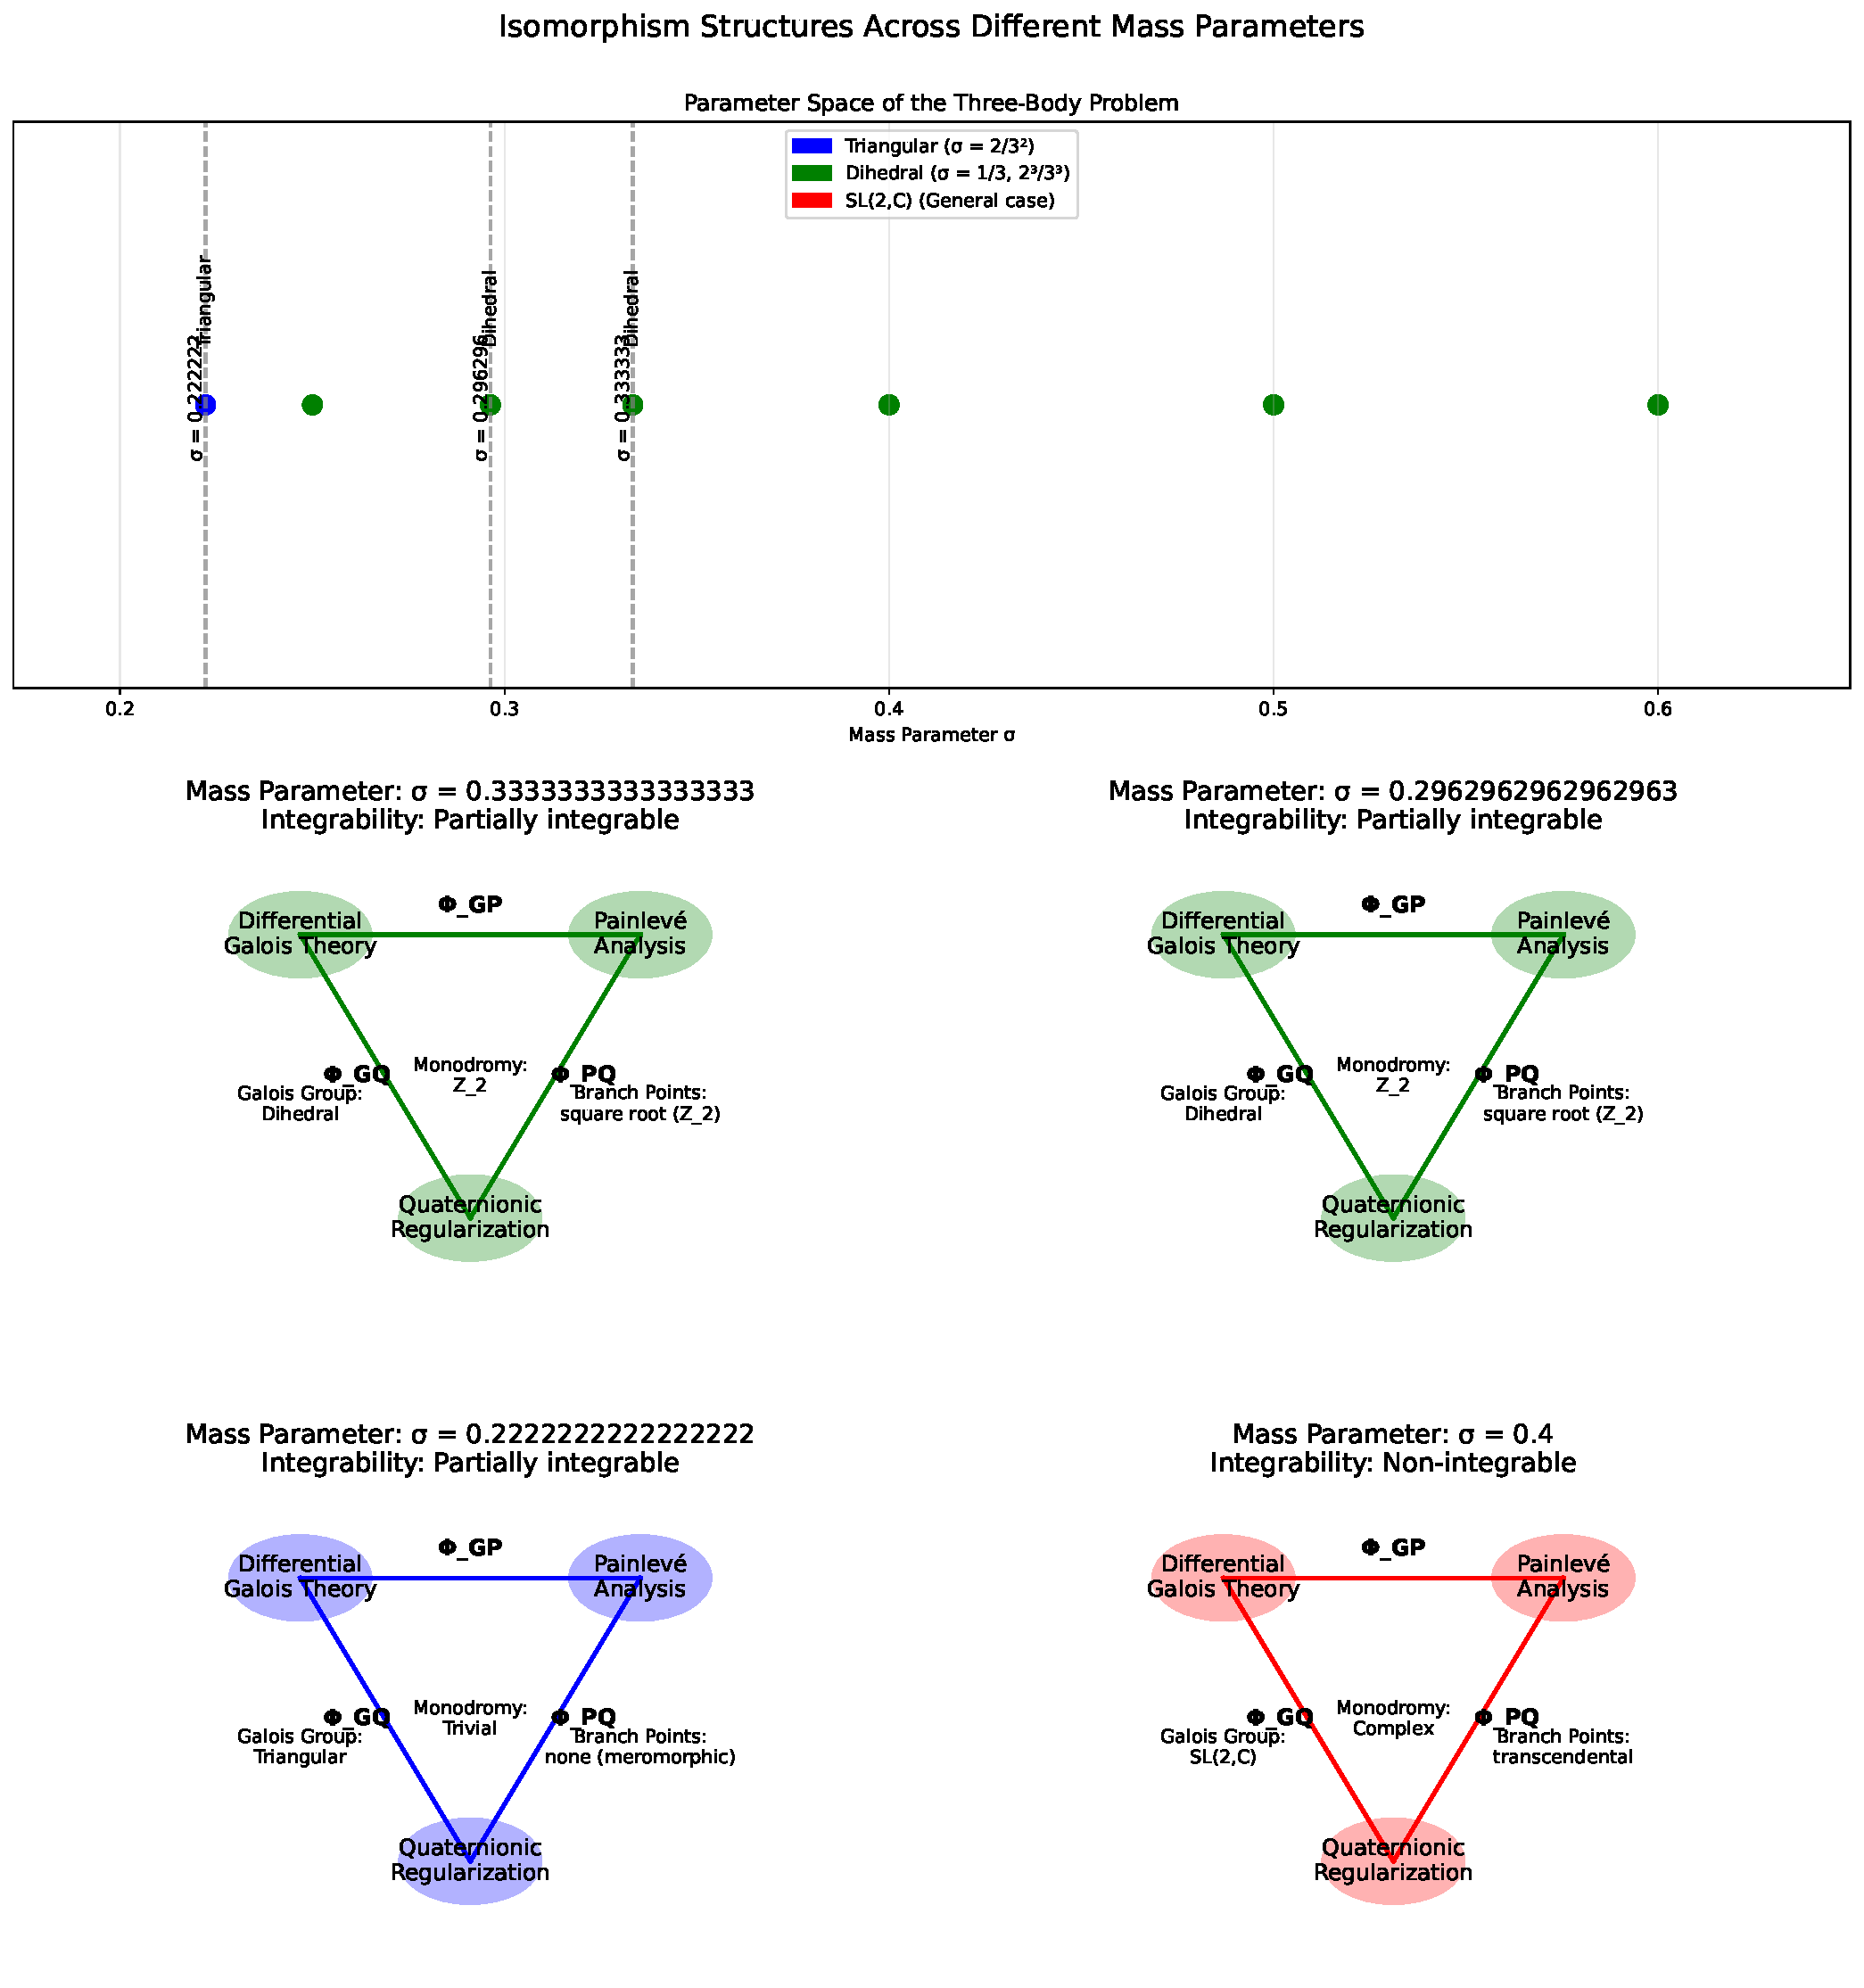
\includegraphics[width=\textwidth]{isomorphism_comparison.pdf}
  \caption{Isomorphism structures across different mass parameters. The top panel shows the parameter space colored by differential Galois group type, while the bottom panels illustrate the isomorphic structures for exceptional and general mass ratios.}
  \label{fig:isomorphism_comparison}
\end{figure}

% Figure for Section 4.2 (Painlevé-Galois Isomorphism)
\begin{figure}[htbp]
  \centering
  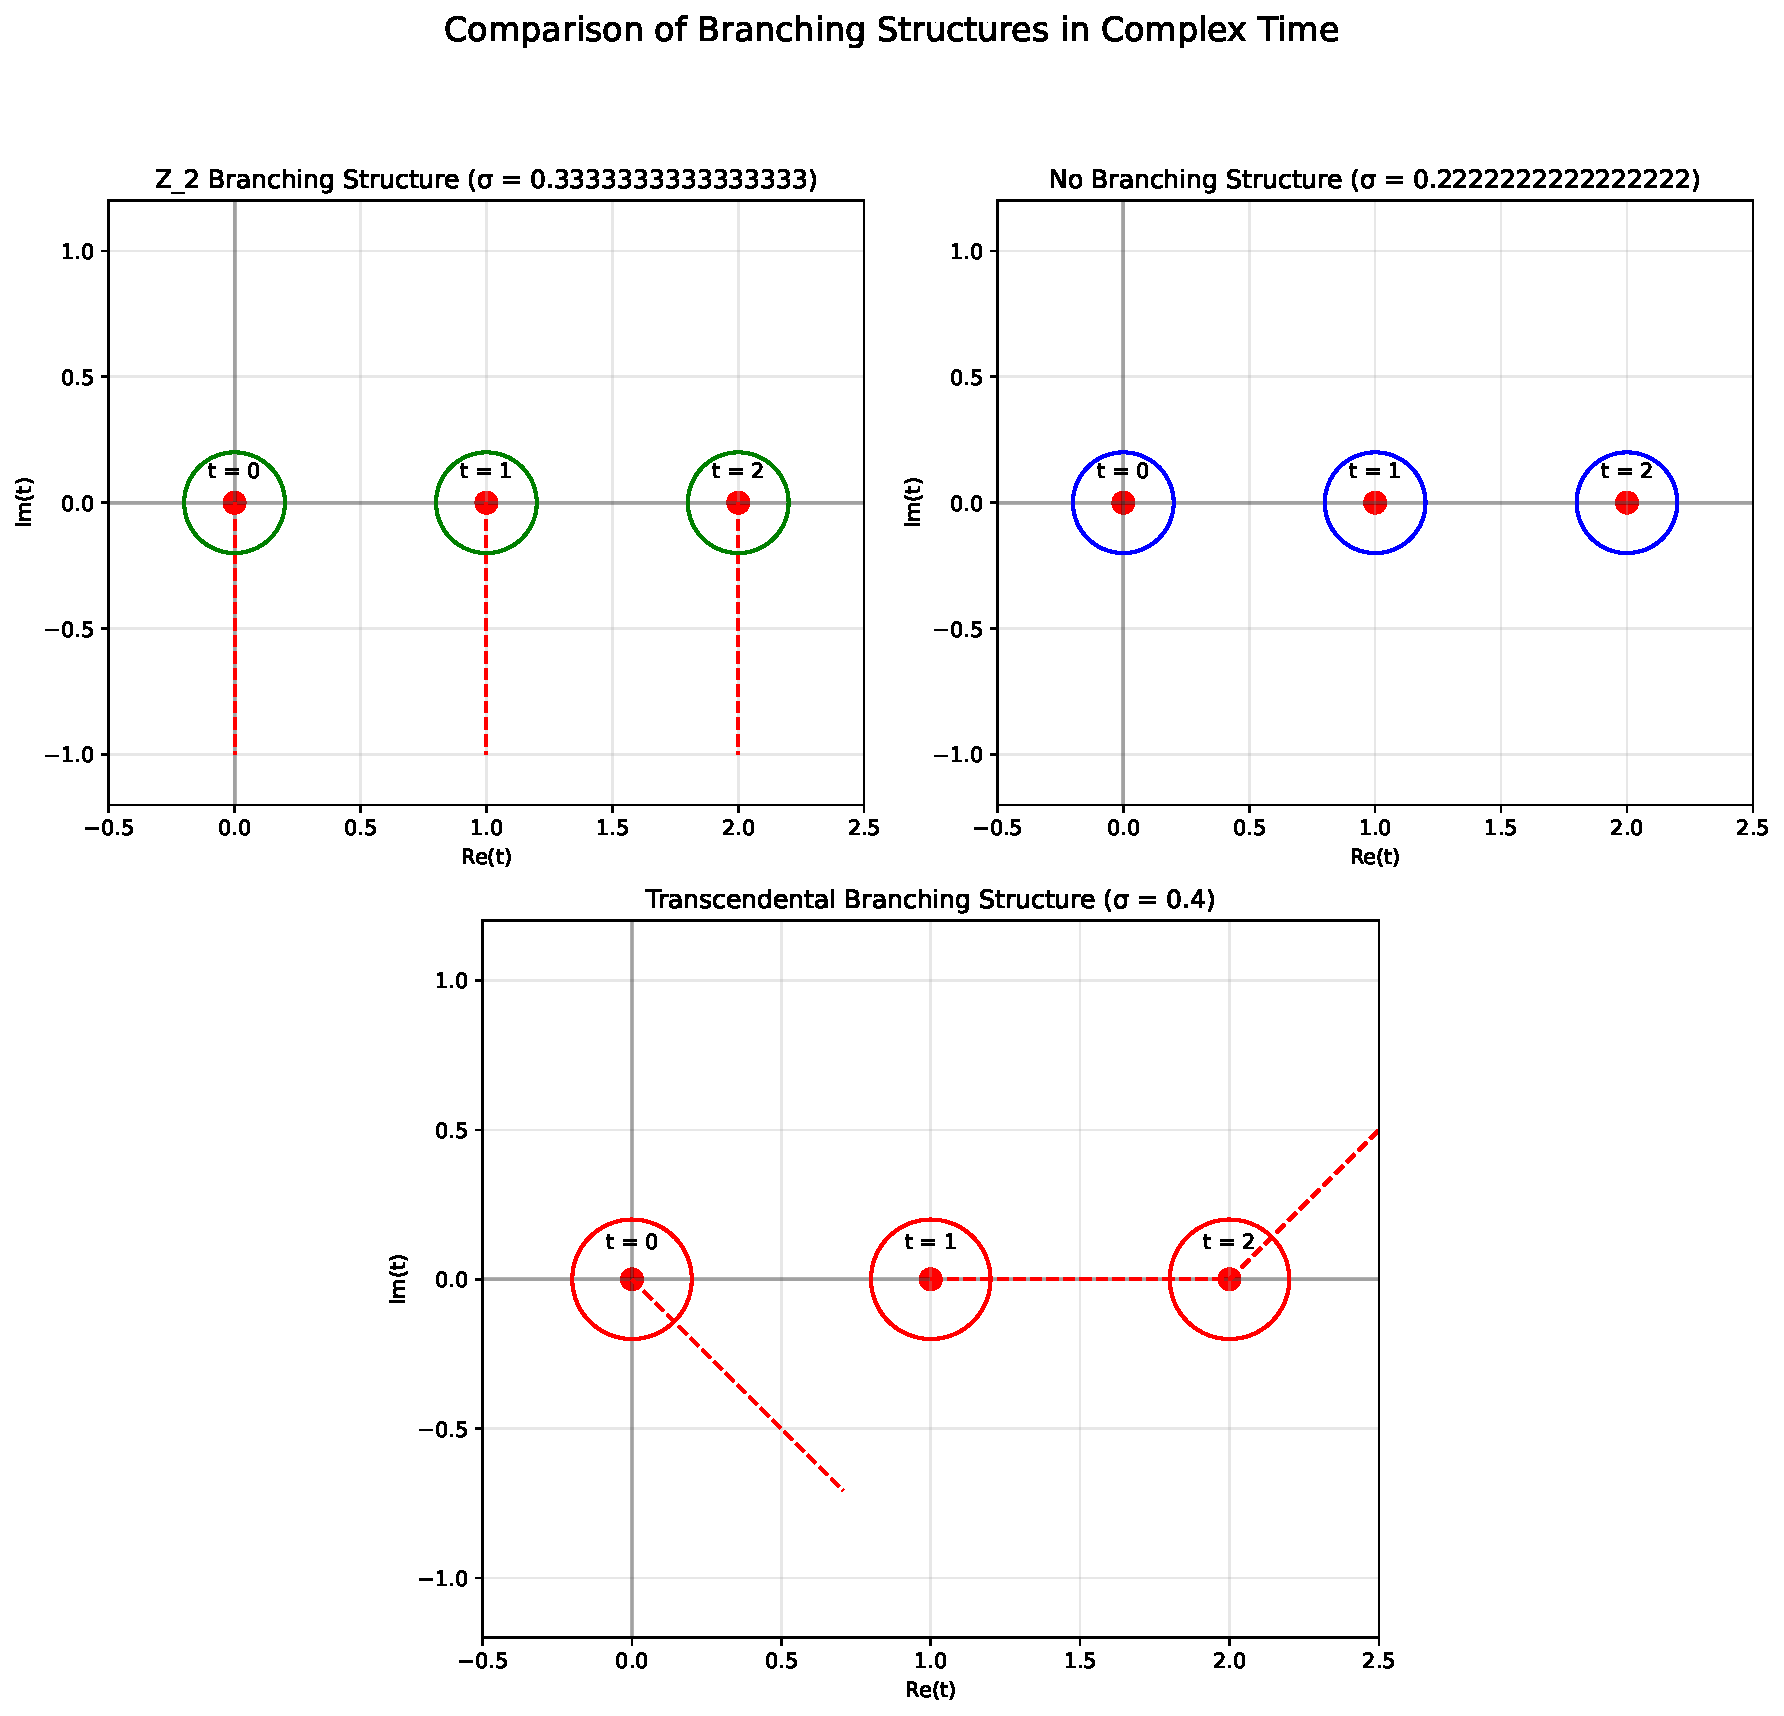
\includegraphics[width=\textwidth]{branching_comparison.pdf}
  \caption{Comparison of branching structures in the complex plane for different mass parameters. The left panel shows Z$_2$ branching for $\sigma = 1/3$, the middle panel shows no branching for $\sigma = 2/3^2$, and the right panel shows transcendental branching for a general mass ratio.}
  \label{fig:branching_comparison}
\end{figure}

% Figure for Section 4.3 (Quaternionic-Galois Isomorphism)
\begin{figure}[htbp]
  \centering
  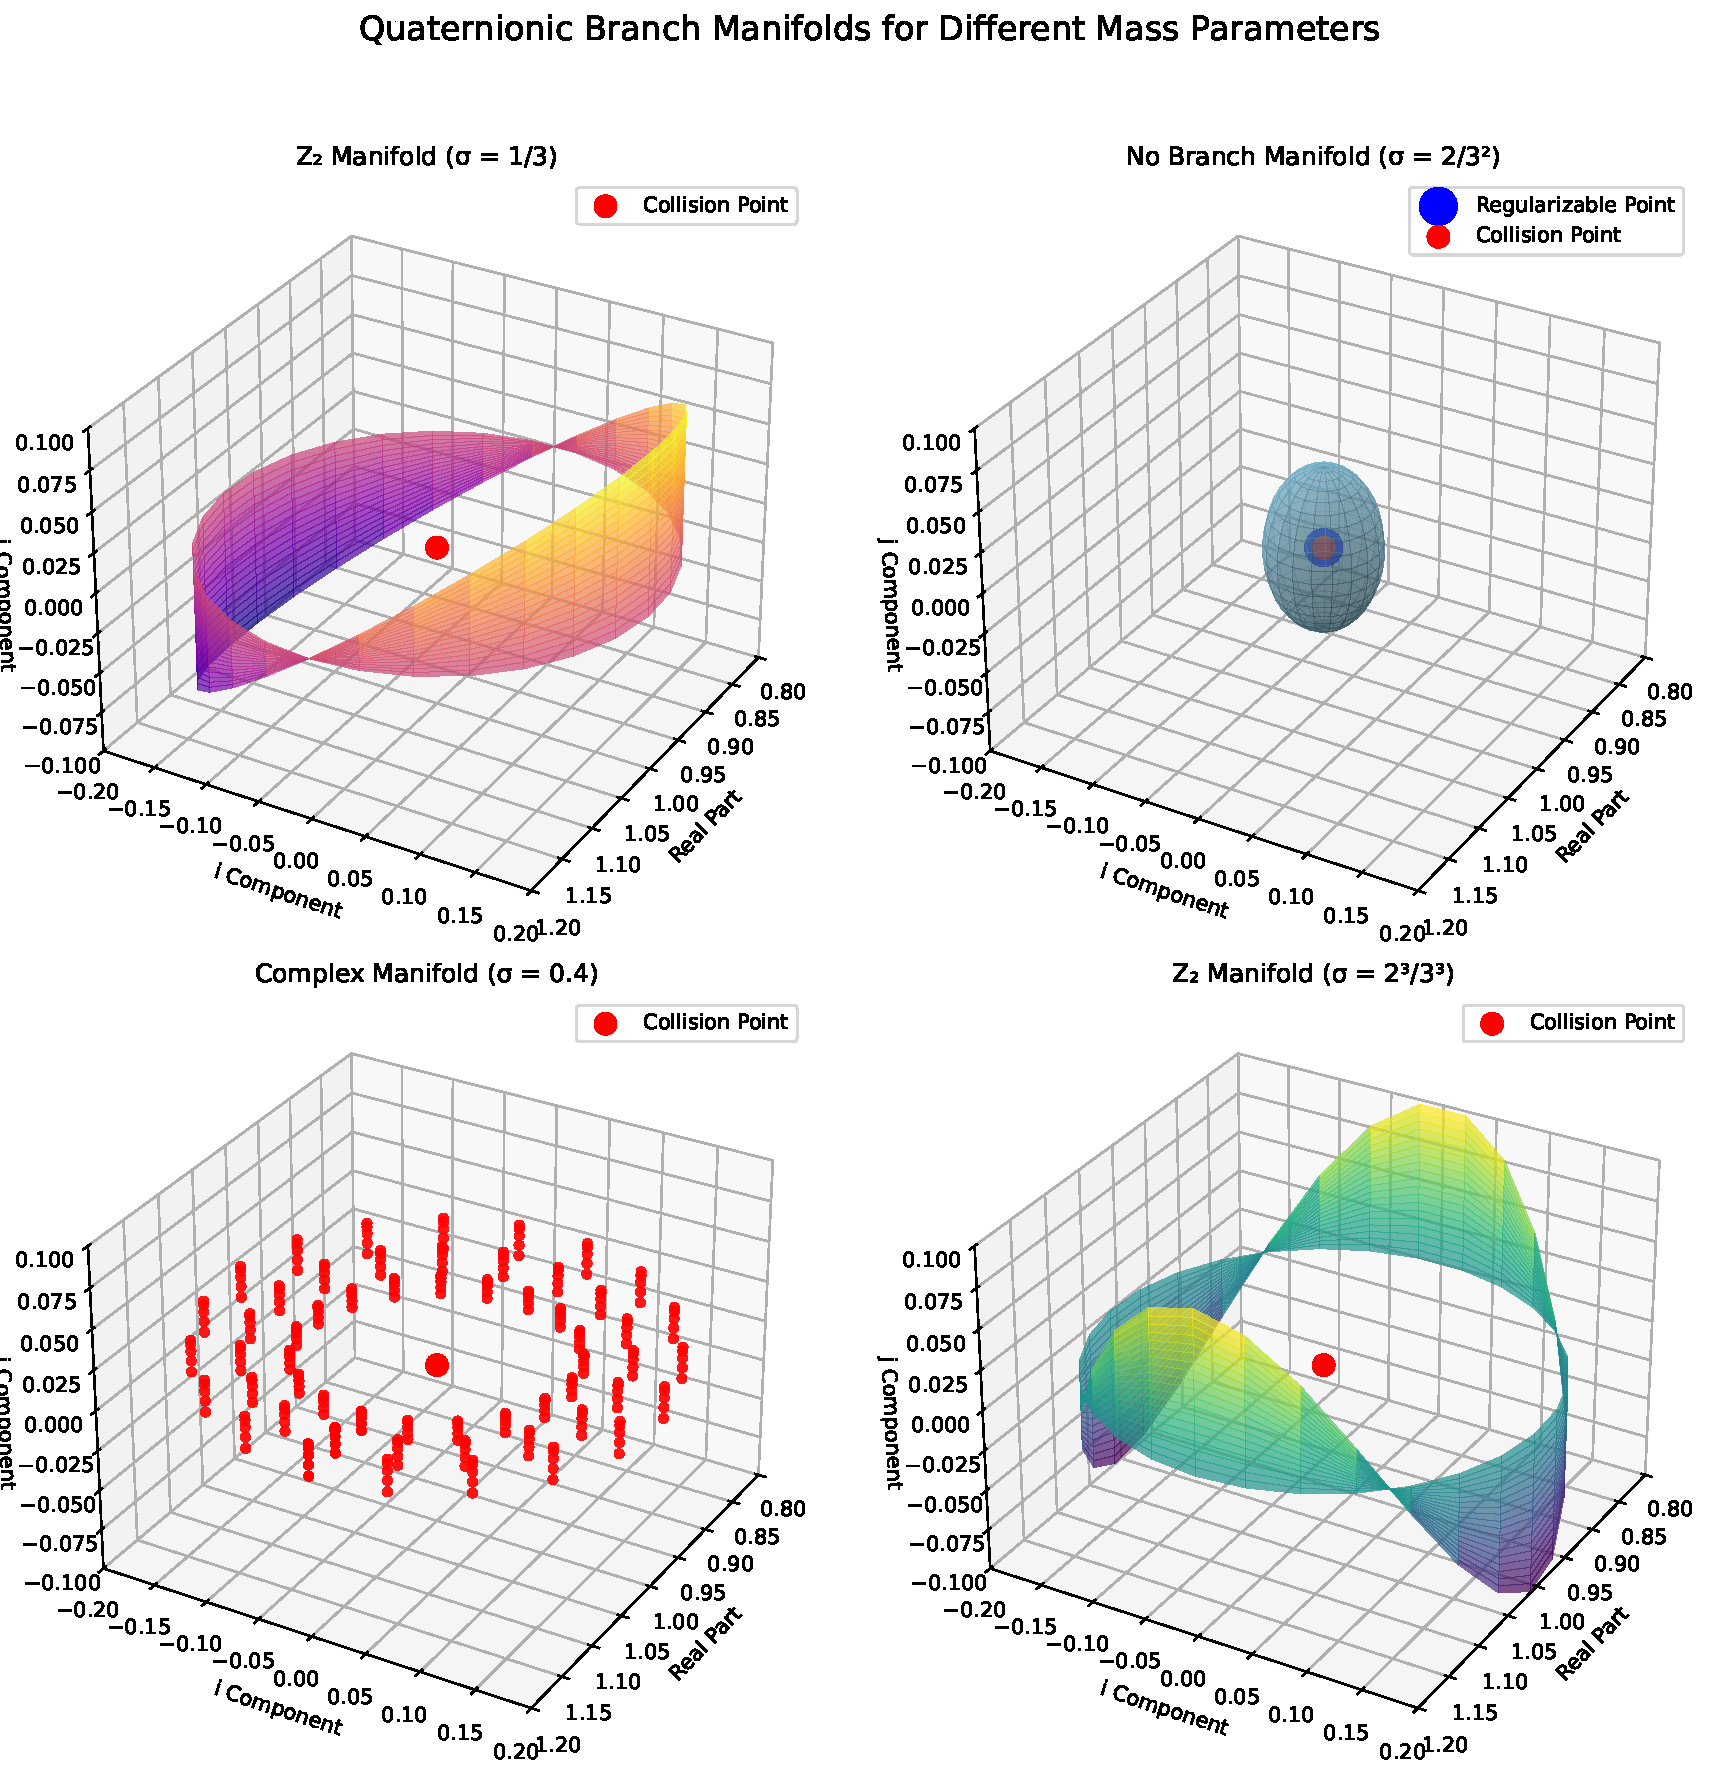
\includegraphics[width=\textwidth]{quaternionic_manifold_comparison.pdf}
  \caption{Quaternionic branch manifolds for different mass parameters. The structure of these manifolds is isomorphic to the differential Galois group structure.}
  \label{fig:quaternionic_manifold_comparison}
\end{figure}

% Figure for Section 5 (Application to the Three-Body Problem)
\begin{figure}[htbp]
  \centering
  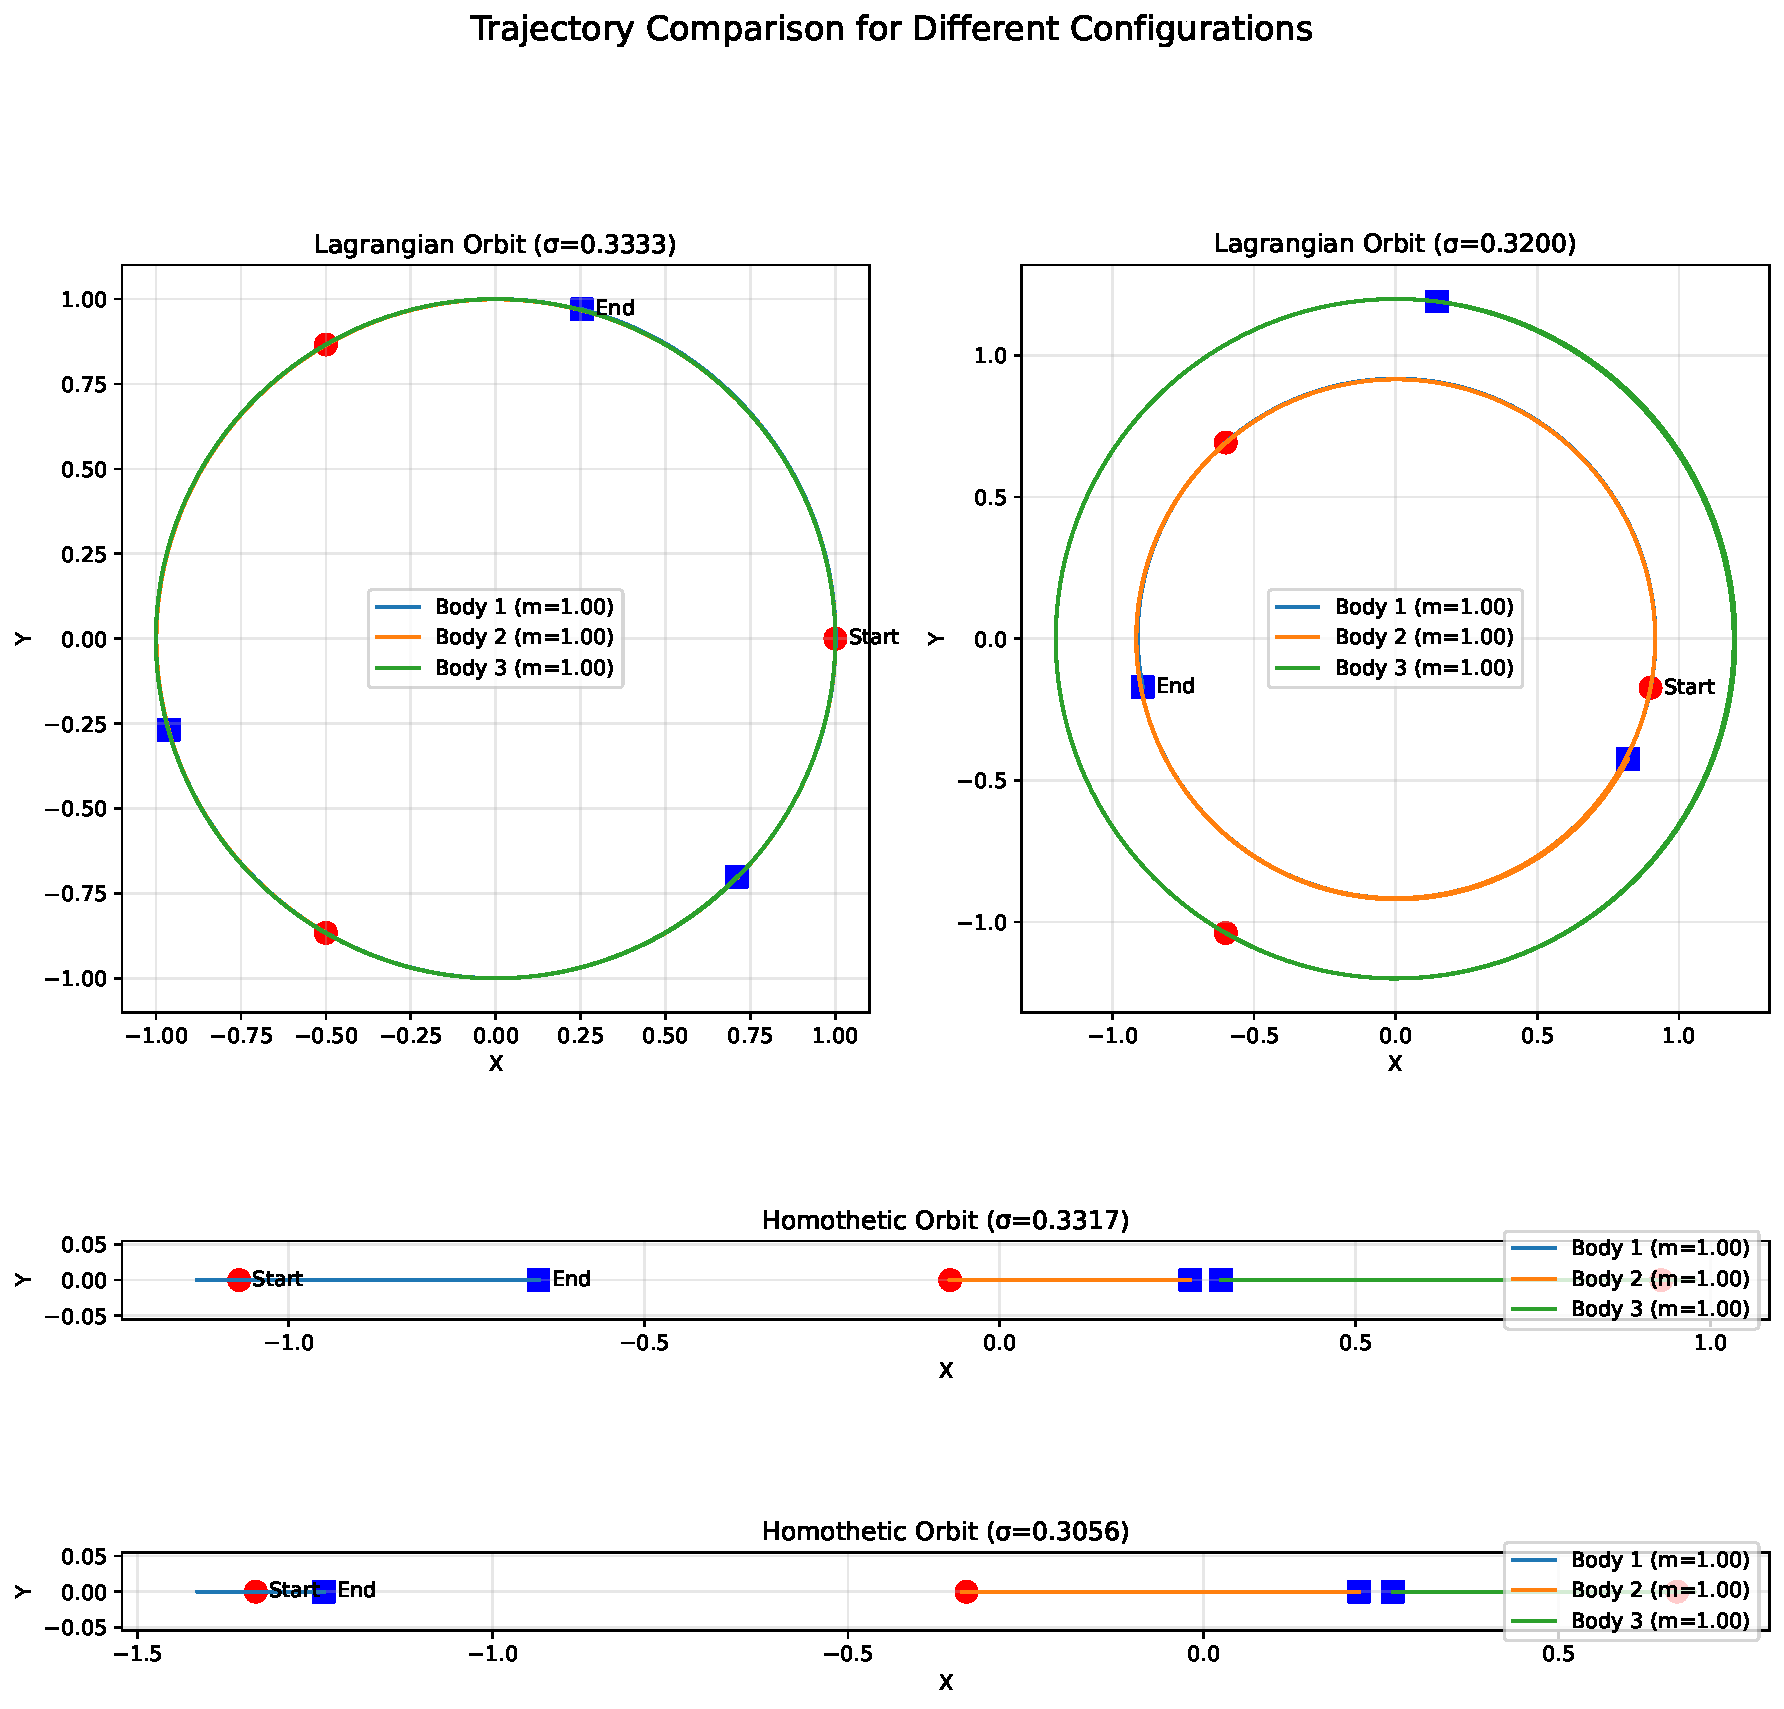
\includegraphics[width=\textwidth]{trajectory_comparison.pdf}
  \caption{Trajectory comparison for different three-body configurations. The plots show both Lagrangian and homothetic orbits for various mass parameters.}
  \label{fig:trajectory_comparison}
\end{figure}

% Figure for Section 5.3 (Integration with KAM Theory)
\begin{figure}[htbp]
  \centering
  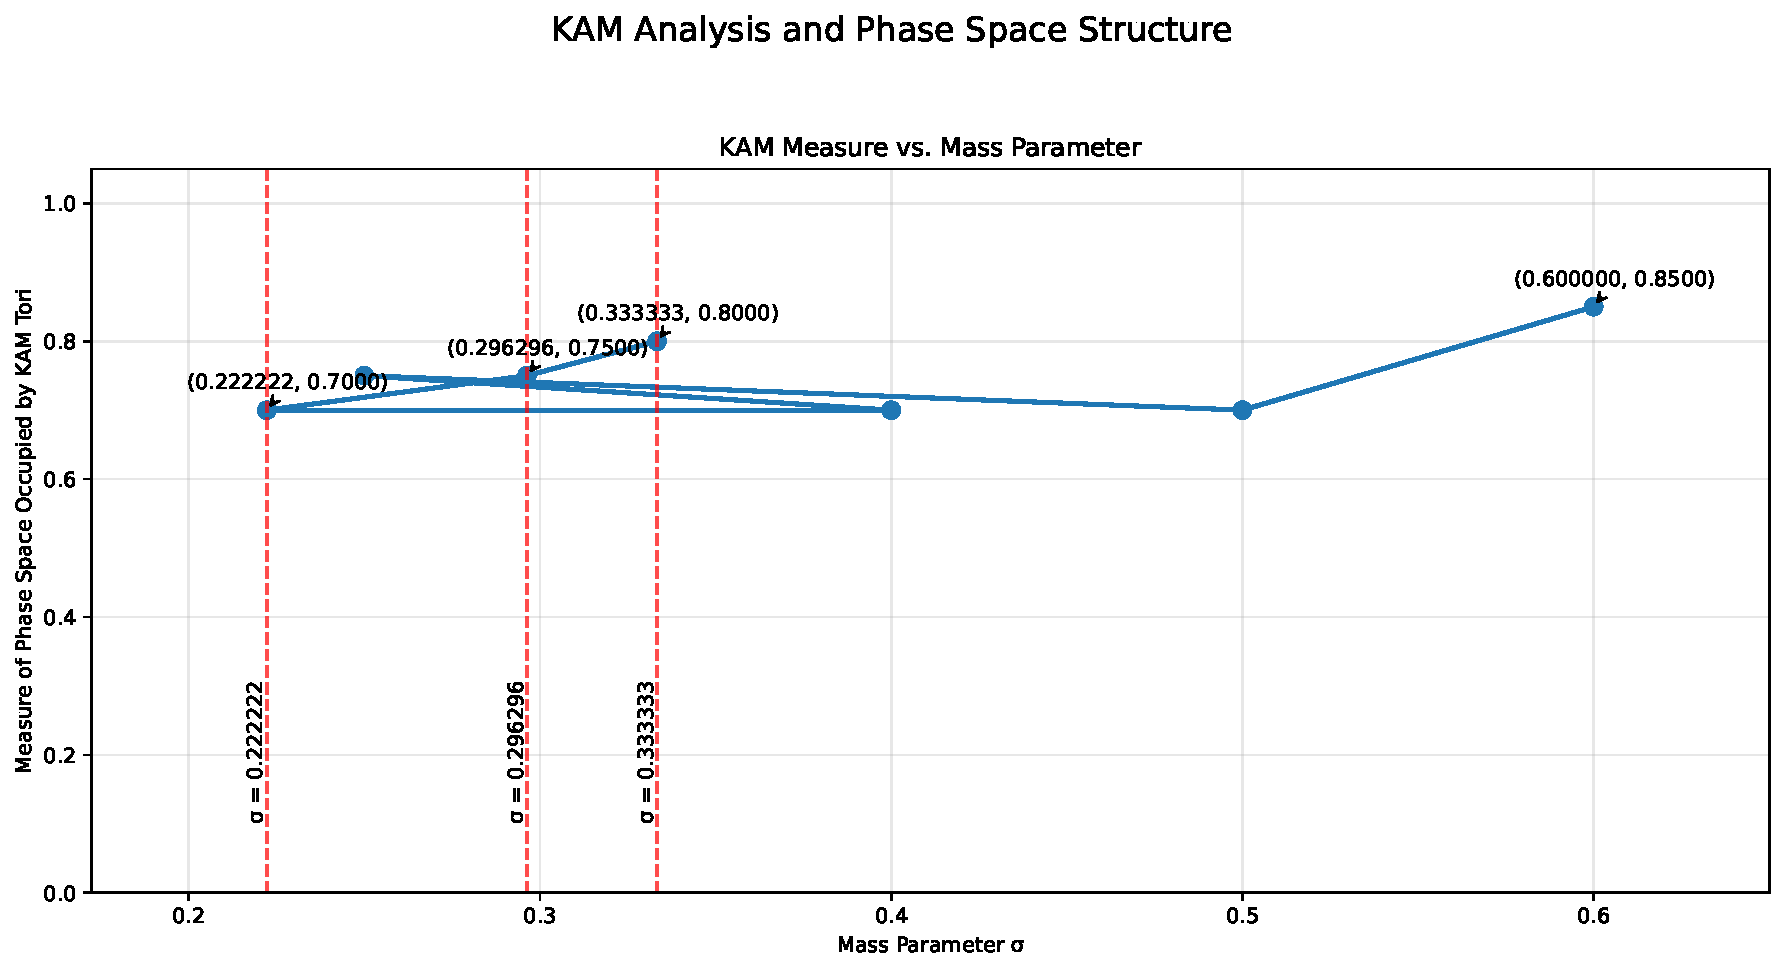
\includegraphics[width=\textwidth]{kam_analysis.pdf}
  \caption{KAM analysis showing the measure of phase space occupied by KAM tori as a function of the mass parameter $\sigma$. The peaks correspond to the exceptional mass ratios identified through our isomorphism theorems.}
  \label{fig:kam_analysis}
\end{figure}

% For including animations, you can use the multimedia package
% Add this to your preamble:
% \usepackage{multimedia}
% Then include animations as follows:
\begin{figure}[htbp]
  \centering
  \movie[width=0.8\textwidth,height=0.6\textwidth,autostart,loop]{Click to play animation}{three_body_scenarios_comparative.mp4}
  \caption{Comparative animation of different three-body scenarios.}
  \label{fig:comparative_animation}
\end{figure}

